\documentclass[tikz,border=4mm]{standalone}
\usepackage[T1]{fontenc}
\usepackage{lmodern}
\usetikzlibrary{arrows.meta,positioning,calc}
\begin{document}
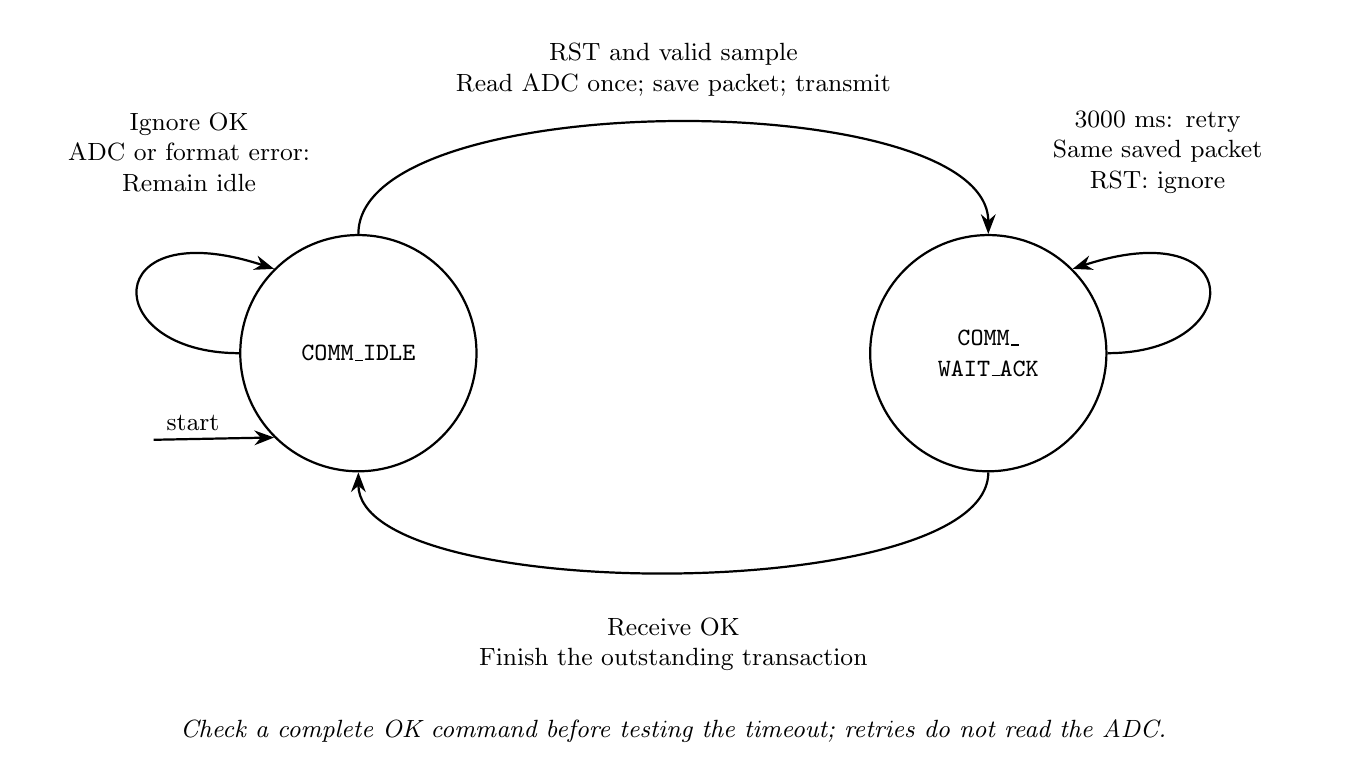
\begin{tikzpicture}[
 font=\small,
 state/.style={circle,draw,thick,minimum size=30mm,align=center,inner sep=1mm,font=\small\bfseries},
 labelbox/.style={align=center,font=\small,inner sep=2mm,fill=white},
 flow/.style={-{Stealth[length=2.5mm]},thick},
 block/.style={draw,rounded corners=2mm,thick,align=center,text width=39mm,minimum height=20mm,inner sep=3mm}]

\node[state] (idle) at (-4,0) {\texttt{COMM\_IDLE}};
\node[state] (wait) at (4,0) {\texttt{COMM\_}\\\texttt{WAIT\_ACK}};
\draw[flow] (-6.6,-1.1) -- (idle.south west);
\node[font=\small,above] at (-6.1,-1.1) {start};
\draw[flow] (idle.north) .. controls (-4,3.4) and (4,3.4) .. (wait.north);
\node[labelbox] at (0,3.6) {RST and valid sample\\Read ADC once; save packet; transmit};
\draw[flow] (wait.south) .. controls (4,-3.2) and (-4,-3.2) .. (idle.south);
\node[labelbox] at (0,-3.7) {Receive OK\\Finish the outstanding transaction};
\draw[flow] (idle.west) .. controls (-7.3,0) and (-7.3,1.8) .. (idle.north west);
\node[labelbox,text width=37mm] at (-6.15,2.55) {Ignore OK\\ADC or format error:\\Remain idle};
\draw[flow] (wait.east) .. controls (7.3,0) and (7.3,1.8) .. (wait.north east);
\node[labelbox,text width=37mm] at (6.15,2.55) {3000 ms: retry\\Same saved packet\\RST: ignore};
\node[align=center,font=\small\itshape] at (0,-4.8) {Check a complete OK command before testing the timeout; retries do not read the ADC.};

\end{tikzpicture}
\end{document}
